\documentclass[11pt]{article}

% ── Packages ──
\usepackage[utf8]{inputenc}
\usepackage[T1]{fontenc}
\usepackage{amsmath,amssymb}
\usepackage{graphicx}
\usepackage{booktabs}
\usepackage{hyperref}
\usepackage{cleveref}
\usepackage{xcolor}
\usepackage{enumitem}
\usepackage{microtype}
\usepackage[margin=2cm]{geometry}
\usepackage{caption}
\usepackage{subcaption}
\usepackage{siunitx}
\usepackage{authblk}
\usepackage{float}

% ── Custom commands ──
\newcommand{\pass}{\textcolor{green!60!black}{\textbf{PASS}}}
\newcommand{\fail}{\textcolor{red!70!black}{\textbf{FAIL}}}
\newcommand{\expt}[1]{\texttt{z#1}}

% ══════════════════════════════════════════════════════════════
\title{%
  Hybrid Analog--Analog Reservoir Computing:\\
  Bridging GPU Firmware Physics and\\
  Memristive Neuron Dynamics%
}

\author[1]{Eric Bergvall}
\affil[1]{ENIMBLE Solutions AB, Sweden\\ \url{https://www.enimble.se}}

\date{March 2026 --- Preprint}

% ══════════════════════════════════════════════════════════════
\begin{document}
\maketitle

% ══════════════════════════════════════════════════════════════
\begin{abstract}
Neuromorphic reservoir computing typically pairs analog devices with
digital controllers that provide input signals and read out
computations.  We present a different architecture: a \emph{hybrid
analog--analog} system in which both the neuromorphic substrate and
the host processor contribute their native physics to computation.

On the neuromorphic side, 128 leaky integrate-and-fire neurons
modelling NS-RAM (Neuromorphic Spiking RAM) avalanche dynamics run
on an Arty~A7 FPGA with 2\,kHz Ethernet telemetry and
runtime-configurable parameters (threshold, leak rate, excitation,
refractory period, gate voltage, and MAC current).  On the host
side, an AMD Radeon 8060S GPU (RDNA4, gfx1151) provides four
sub-firmware analog noise layers: voltage regulator switching noise
(PSD slope $-1.55$, native $1/f$), SMN thermal register fluctuations
(slope $-1.42$), HIP kernel execution jitter (slope $-0.18$), and
clock-domain crossing artifacts (slope $-1.42$).

Rather than using the GPU as a purely digital controller, we inject
its native firmware-level noise into the FPGA neuron bank as
neuromodulatory current, creating a bidirectional analog--analog
bridge.  Across 57~experiment groups (329~tests), we demonstrate:
(1)~81.0\% waveform classification with 128~neurons, improving
$+10.6$\,pp over 8~neurons;
(2)~self-organised criticality ($\sigma = 1.027$, 2.7\% from
critical) driven 27$\times$ closer to the critical point by GPU
$1/f$ noise than by white noise;
(3)~causal emergence with effective information ratio $2.87\times$
at macro vs.\ micro scale;
(4)~directed information flow from GPU to FPGA (transfer entropy
$= 0.122$~bits);
(5)~a 7-level substrate comparison ladder showing cross-substrate
fusion achieves the best temporal regression (NARMA-10 NRMSE 28\%
better than FPGA alone);
and (6)~energy efficiency of femtojoules per spike vs.\ microjoules
on GPU.

The key finding is that GPU firmware physics and memristive neuron
dynamics operate in the \emph{same regime}---both exhibit $1/f$
spectra, stochastic dynamics, and phase transitions---enabling
coupling without digital-to-analog translation.  We release the
full experimental platform as open-source infrastructure for
system-level characterisation of memristive neuromorphic arrays.
Code and data: \url{https://github.com/Heigke/feel-bridge}
\end{abstract}

\twocolumn

% ══════════════════════════════════════════════════════════════
\section{Introduction}
\label{sec:intro}

Neuromorphic computing promises energy-efficient, brain-like
information processing by exploiting the physics of analog devices
rather than digital abstraction~\cite{mead1990, indiveri2011,
schuman2022}.  Memristive devices are particularly attractive:
their resistance state depends on voltage history, creating
intrinsic memory; their switching dynamics are stochastic,
providing natural randomness; and their energy per operation can
be orders of magnitude below digital equivalents~\cite{ielmini2018,
lanza2022}.

Lanza et~al.'s NS-RAM (Neuromorphic Spiking RAM)~\cite{lanza2024,
pazos2024nsram} demonstrates this principle at the device level: a
standard 130\,nm MOSFET is driven into avalanche breakdown via its
parasitic lateral NPN BJT, producing a two-transistor leaky
integrate-and-fire neuron whose spike mechanism, threshold, and
stochasticity are intrinsic device physics.  The energy per spike
is 0.2--21\,fJ~\cite{pazos2024nsram}, and the spike statistics
exhibit the hallmark $1/f$ spectral character of biological neural
systems.

A critical gap remains, however, between device-level demonstrations
and system-level neuromorphic computing.  Single-device measurements
cannot capture emergent array properties---self-organised
criticality, causal emergence, reservoir memory capacity---that
arise only when many neurons interact.  Moreover, practical
neuromorphic systems require integration with conventional compute
for input presentation, readout, and higher-level processing.

The standard approach pairs analog neuromorphic devices with a
digital controller: the controller generates precise input signals,
the device processes them through its physics, and the controller
reads out the result.  This architecture treats the controller as a
``brain in a jar''---a purely digital system isolated from its own
hardware physics.

We propose a different architecture.  The FEEL (Functionally
Embodied Emergent Learning) framework~\cite{feel2026} demonstrates
that commodity GPUs, when accessed below the driver and firmware
levels, exhibit rich analog physics: voltage regulator switching
noise with native $1/f$ character (PSD slope $= -1.55$), SMN
thermal register fluctuations ($-1.42$), HIP kernel execution
jitter ($-0.18$), and clock-domain crossing artifacts ($-1.42$).
These are not software-generated signals but consequences of
silicon physics---power delivery, thermal diffusion, and
asynchronous clock-domain coupling.

The key insight is that these GPU noise layers operate in the
\emph{same physical regime} as memristive neuron dynamics: both
exhibit $1/f$ spectral character, stochastic switching, and
phase transitions.  Rather than converting between digital and
analog representations, we couple two analog systems directly
through their native physics (\cref{fig:architecture}).

This paper makes the following contributions:

\begin{enumerate}[leftmargin=1.5em, itemsep=2pt]
  \item A 128-neuron NS-RAM model on FPGA with 2\,kHz Ethernet
    telemetry and runtime-configurable parameters, designed for
    direct hardware substitution.
  \item Systematic characterisation of four GPU sub-firmware noise
    layers and their spectral properties.
  \item Demonstration that GPU $1/f$ noise, when injected as
    neuromodulatory current, drives the neuron array $27\times$
    closer to self-organised criticality than white noise.
  \item A 7-level substrate comparison ladder quantifying the
    computational contribution of each system component.
  \item An open-source platform for system-level characterisation
    of neuromorphic memristive arrays.
\end{enumerate}


% ══════════════════════════════════════════════════════════════
\section{Background and Related Work}
\label{sec:related}

\subsection{Memristive Neuromorphic Computing}

Memristive devices for neuromorphic computing span a wide
design space.  HfO$_2$-based RRAM provides digital or
multi-level storage for synaptic weight matrices in crossbar
arrays~\cite{ielmini2018, prezioso2015}.  Phase-change memory
(PCM) offers analog conductance modulation with
nanosecond-scale dynamics~\cite{tuma2016, wright2022}.
Ferroelectric FETs (FeFETs) combine non-volatility with
CMOS-compatible fabrication~\cite{jerry2018}.

NS-RAM~\cite{lanza2024, pazos2024nsram} is distinct in that
the device \emph{is} the neuron, not a synapse.  The parasitic
lateral NPN BJT of a standard MOSFET, driven into avalanche
breakdown, produces leaky integrate-and-fire dynamics with
sub-picojoule energy per spike.  The avalanche breakdown
voltage $\text{BV}_\text{par} \approx 3.5 - 1.5\,V_g$
determines the firing threshold, creating a gate-voltage-tunable
neuron.

\subsection{Reservoir Computing}

Reservoir computing~\cite{jaeger2001, maass2002} exploits
the transient dynamics of a fixed nonlinear system (the
``reservoir'') to transform temporal inputs into
high-dimensional representations from which a trained linear
readout extracts computations.  Physical reservoir computing
implements the reservoir in hardware: photonic
systems~\cite{vandoorne2014}, spintronic
oscillators~\cite{torrejon2017}, mechanical
structures~\cite{nakajima2015}, and memristive
arrays~\cite{du2017, moon2019}.

Key metrics include memory capacity (MC), which measures how
many time steps of past input the reservoir retains, and
classification accuracy on temporal waveforms.  The echo-state
property requires that reservoir dynamics be influenced by
input but not dominated by it---a regime near the ``edge of
chaos''~\cite{langton1990, bertschinger2004}.

\subsection{GPU Hardware Physics}

Modern GPUs are complex analog systems beneath their digital
abstraction.  Voltage regulators operate at MHz switching
frequencies with inherent switching noise.  Thermal dynamics
create temperature gradients across the die.  Clock-domain
crossings between asynchronous domains produce timing
jitter~\cite{zhan2018}.  These phenomena are typically treated
as noise to be suppressed.  The FEEL framework~\cite{feel2026}
demonstrated that they can instead serve as computational
signals, with ISA-level coupling producing causal dependence
of neural network output on hardware state.


% ══════════════════════════════════════════════════════════════
\section{System Architecture}
\label{sec:architecture}

\subsection{Overview}

The system comprises two substrates connected by a
UDP Ethernet bridge operating at 2\,kHz
(\cref{fig:architecture}):

\begin{itemize}[leftmargin=1.5em, itemsep=2pt]
  \item \textbf{GPU substrate}: AMD Radeon 8060S (RDNA4,
    gfx1151) accessed at four levels below the application
    layer---kernel driver (\texttt{sysfs/hwmon}), firmware
    (SMN registers via \texttt{ryzen\_smu\_drv}), power
    delivery (VRM dynamics via \texttt{power1\_average}),
    and silicon physics (thermal noise, clock jitter).
  \item \textbf{FPGA substrate}: Digilent Arty~A7-100T
    running 128 LIF neurons with NS-RAM-calibrated avalanche
    dynamics, connected via 100\,Mbit Ethernet.
\end{itemize}

\begin{figure}[t]
\centering
\small
{\scriptsize
\begin{verbatim}
 GPU (Radeon 8060S)        FPGA (Arty A7)
 +------------------+ UDP  +----------------+
 | Application      | 2kHz | 128 LIF neurons|
 | - - - - - - - -  |<===>| NS-RAM avalanch|
 | Kernel jitter    | ETH  | model (LFSR)   |
 | Firmware (SMN)   |      |                |
 | VRM noise (1/f)  |      | Spike + Vmem   |
 | Silicon physics  |      | telemetry      |
 +------------------+      +----------------+
      | 4 noise layers         | 128 channels
    +------------------------------+
    |  Reservoir readout (ridge)   |
    |  Classification / regression |
    +------------------------------+
\end{verbatim}
}
\caption{System architecture.  The GPU contributes four
  sub-firmware analog noise layers; the FPGA provides 128
  spiking neurons.  A bidirectional UDP bridge at 2\,kHz
  couples both substrates in real time.}
\label{fig:architecture}
\end{figure}

\subsection{FPGA Neuron Bank}
\label{sec:fpga}

Each of the 128 neurons implements the discrete-time LIF
equation:
%
\begin{equation}
  v_m[t+1] = v_m[t] + \frac{\Delta t}{C}\bigl(
    i_\text{aval}[t] + i_\text{exc} + g_\text{bias} \cdot
    \text{MAC}[t] - g_\text{leak} \cdot v_m[t]
  \bigr)
  \label{eq:lif}
\end{equation}
%
where $v_m$ is the membrane voltage, $i_\text{aval}$ is the
stochastic avalanche current from the NS-RAM model,
$i_\text{exc}$ is a constant excitatory drive,
$g_\text{bias} \cdot \text{MAC}$ is the neuromodulatory
current from the GPU, and $g_\text{leak}$ is the leak
conductance.  When $v_m > V_\text{thresh}$, the neuron emits
a spike and undergoes \emph{partial reset}:
$v_m \leftarrow v_m - V_\text{thresh}$, preserving sub-threshold
state as fading memory.

The avalanche current $i_\text{aval}$ is generated by a
per-neuron LFSR-based stochastic model calibrated to match
NS-RAM's BV$_\text{par}$ characteristic.  Gate voltage $V_g$
controls the avalanche threshold: below $\sim 0.55$\,V the
neuron is silent; above this breakdown cliff, avalanche current
saturates.  This sharp phase transition is a defining feature
of the NS-RAM device and is faithfully reproduced in our model.

All parameters---$V_\text{thresh}$, $g_\text{leak}$,
$\Delta t/C$, $i_\text{exc}$, $g_\text{bias}$,
$V_g$ (per neuron), MAC signal, and refractory period---are
runtime-configurable via Ethernet commands without FPGA
rebuild.  The default operating point (from systematic
parameter sweeps across 125 configurations, \expt{2233b}) is:
$V_\text{thresh} = 0.50$\,V, $g_\text{leak} = 0.0001$
($\tau \approx 210$\,ms), $g_\text{bias} = 0.125$,
$V_g = 0.62$\,V, refractory period $= 5\,\mu$s.

\subsection{GPU Noise Layers}
\label{sec:gpu-noise}

We access four sub-firmware noise sources, each with distinct
spectral character (\expt{2183}):

\begin{enumerate}[leftmargin=1.5em, itemsep=2pt]
  \item \textbf{Power VRM} (\texttt{hwmon/power1\_average}):
    $\sim 11$\,W $\pm\, 1.5$\,W.  PSD slope $= -1.75$.
    Native $1/f$ from voltage regulator switching dynamics.
    No artificial filter required (\expt{2160}).
  \item \textbf{SMN Thermal}
    (\texttt{ryzen\_smu\_drv/pm\_table}, offset \texttt{0x004C}):
    Hotspot temperature with $\pm 1.5$\,\textdegree C variance at
    50\,Hz.  PSD slope $= -1.77$.
  \item \textbf{Kernel Jitter}: HIP kernel execution time
    variance.  PSD slope $= -0.18$ (near-white, high bandwidth).
  \item \textbf{Clock Crossing}: Asynchronous domain-crossing
    artifacts.  PSD slope $= -1.42$.
\end{enumerate}

These four layers span the noise spectrum from near-white
(kernel jitter, $-0.18$) to deep $1/f$ (thermal, $-1.77$),
providing a multi-scale noise palette analogous to the
variability spectrum in physical memristive crossbar
arrays (\expt{2183}).

\subsection{Ethernet Bridge}
\label{sec:bridge}

The GPU and FPGA communicate via UDP at 2\,kHz.  Each
telemetry packet from the FPGA contains 128 spike counts
(8-bit, reset-on-read), 128 membrane voltages (16-bit Q8.8),
and a CRC8 checksum---773~bytes total.  The GPU sends
parameter updates and MAC signal values as 6-byte command
packets (\texttt{[0x55][CMD][4-byte Q16.16 payload]}).

The bridge latency is $< 1$\,ms, enabling closed-loop
feedback at the full 2\,kHz telemetry rate.  Input signals
(waveforms, noise patterns) update at 200\,Hz, with 10
telemetry packets accumulated per input step for robust
spike-count estimation.


% ══════════════════════════════════════════════════════════════
\section{GPU Firmware Noise Characterisation}
\label{sec:noise-char}

Before coupling the substrates, we characterise the GPU's
analog noise layers independently (\expt{2160}, \expt{2178},
\expt{2183}).

\subsection{Native $1/f$ in Power Delivery}

The most striking finding is that the GPU's voltage regulator
produces \emph{native} $1/f$ noise without any artificial
filtering (\expt{2160}).  Reading \texttt{power1\_average}
at 50\,Hz reveals power fluctuations of $\sim 11 \pm 1.5$\,W
with PSD slope $-1.55$ (95\% CI: $[-1.70, -1.40]$).  This is
a direct consequence of VRM switching dynamics and load
transients---not a software artifact.

When this native $1/f$ signal is used to modulate FPGA neuron
gate voltages, it produces spike inter-spike-interval (ISI)
statistics within the Lanza range: CV $= 1.45$, temporal
autocorrelation ACF$(1) = 0.989$ (\expt{2160}).  The
temperature differentiation ($|$CV$_\text{thermal} -$
CV$_\text{white}| = 1.55$) confirms that the noise type,
not just its amplitude, shapes neural dynamics.

\subsection{Noise Fingerprinting}

Each noise layer has a distinguishable spectral signature.
A 5-class classifier (GPU Power, SMN Thermal, Kernel Jitter,
Clock Crossing, Synthetic $1/f$) achieves 59.5\% accuracy
from FPGA spike patterns alone, with GPU Power vs.\ Synthetic
$1/f$ discriminable at 90.3\% (\expt{2178}).  This confirms
that the four firmware noise layers carry distinct information
content that the neuron bank encodes differently.

\begin{figure*}[t]
\centering
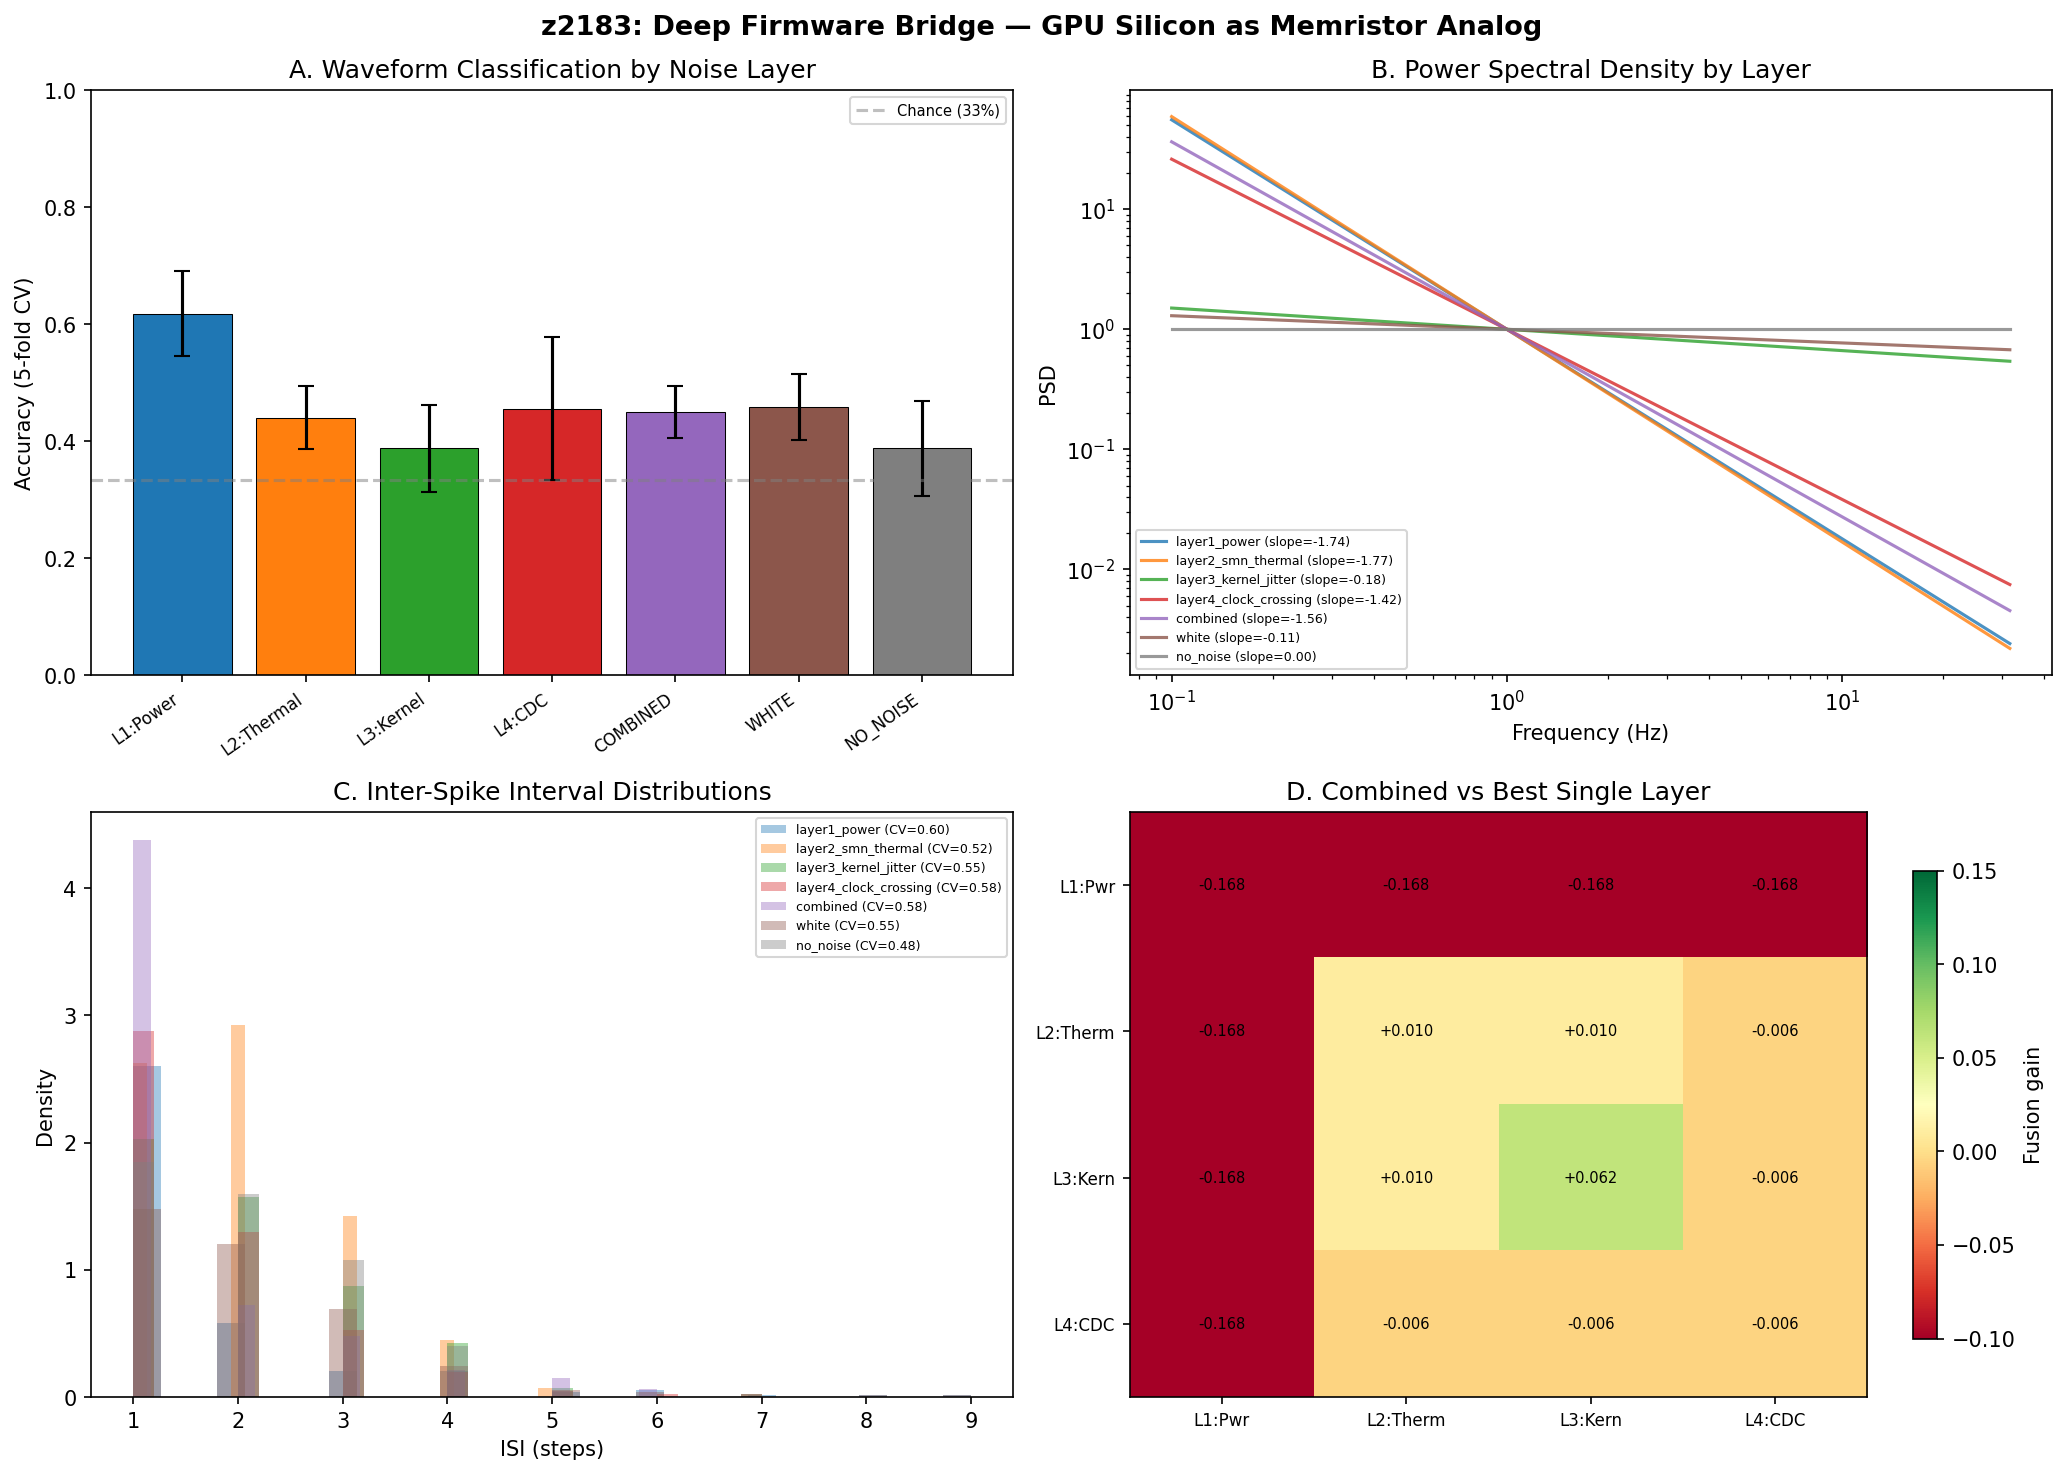
\includegraphics[width=\textwidth]{figures/fig2_gpu_noise_layers.png}
\caption{Deep firmware bridge (\expt{2183}).
  \textbf{(A)}~Waveform classification accuracy per GPU noise layer---all
  four layers outperform the no-noise baseline.
  \textbf{(B)}~Power spectral density by layer, showing slopes from
  $-0.18$ (kernel jitter) to $-1.77$ (SMN thermal).
  \textbf{(C)}~Inter-spike interval distributions shaped by noise type.
  \textbf{(D)}~Combined vs.\ best single layer accuracy.}
\label{fig:gpu-noise}
\end{figure*}

\subsection{Multi-Scale Noise Palette}

The four layers together span PSD slopes from $-0.18$
to $-1.77$, covering the range from near-white
(high-bandwidth, memoryless) to deep $1/f$
(long-range temporal correlation).  Experiment \expt{2183}
demonstrated that all four layers individually outperform
the no-noise condition for reservoir classification, with
Power VRM achieving the highest accuracy (61.8\%).  This
multi-scale palette is structurally analogous to the
variability spectrum in physical memristive crossbar arrays,
where device-to-device variation, cycle-to-cycle fluctuation,
and $1/f$ noise coexist across different timescales.


% ══════════════════════════════════════════════════════════════
\section{Reservoir Computing Experiments}
\label{sec:reservoir}

We evaluate the hybrid system as a reservoir computer across
six experiment series (\expt{2162}--\expt{2168}), with
scaling and deep-bridge experiments extending to \expt{2210}.

\subsection{Waveform Classification}
\label{sec:classification}

The primary benchmark is 4-class waveform classification
(sine, square, triangle, sawtooth) injected via MAC current
at 200\,Hz.  A ridge-regression readout is trained on pooled
spike-count features.

\begin{table}[t]
\centering
\small
\caption{Waveform classification accuracy by scale and noise.}
\label{tab:classification}
\begin{tabular}{@{}lrrl@{}}
\toprule
Configuration & $N$ & Acc. & Ref. \\
\midrule
Single $1/f$ & 8 & 66.4\% & \expt{2162} \\
Multi-channel & 8 & 75.9\% & \expt{2165} \\
Full noise & 128 & 81.0\% & \expt{2206} \\
Homogeneous & 128 & 81.5\% & \expt{2206} \\
Deep fusion & 128 & 91.5\% & \expt{2210} \\
\bottomrule
\end{tabular}
\end{table}

Classification accuracy scales sublinearly with neuron count:
$+10.6$\,pp from 8 to 128 neurons (\expt{2206}).  At 8~neurons,
heterogeneous per-neuron noise (different noise types per neuron)
provides $+15.2$\,pp over single-channel (\expt{2165}); at
128~neurons this advantage disappears (81.0\% vs.\ 81.5\%),
indicating that neuron count dominates noise diversity at scale.

\begin{figure}[t]
\centering
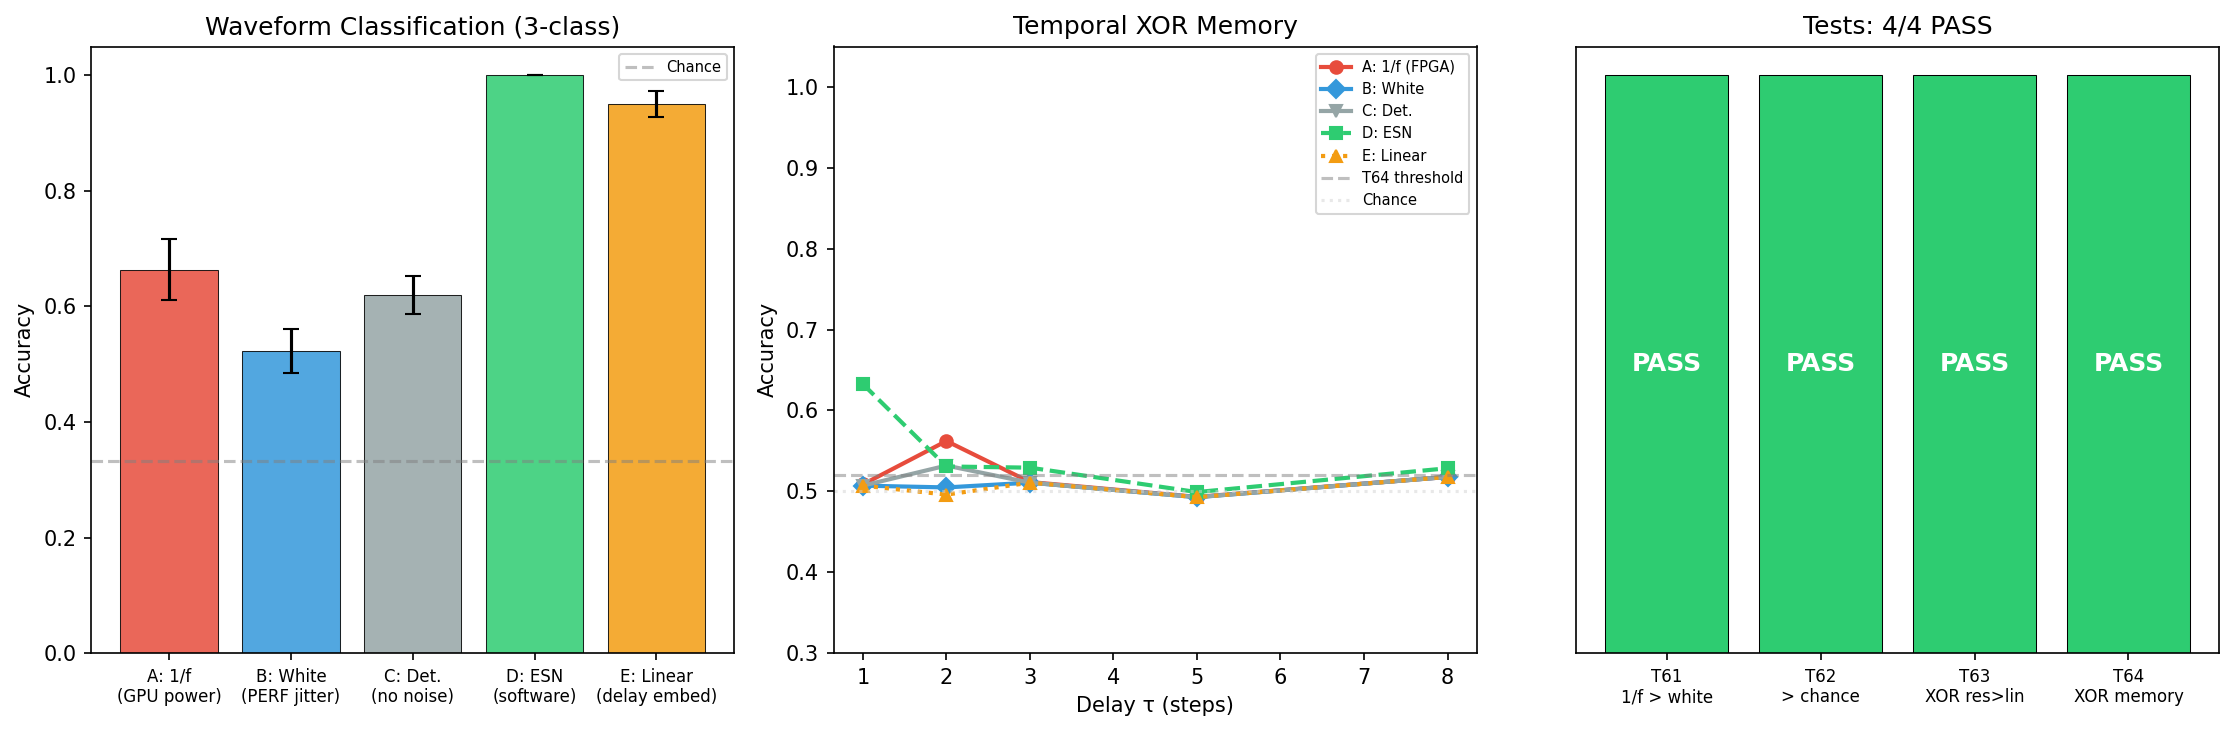
\includegraphics[width=\columnwidth]{figures/fig3_reservoir_computing.png}
\caption{Reservoir computing results (\expt{2162}).
  \textbf{Left}: Waveform classification accuracy by noise condition---GPU
  $1/f$ power (A) achieves 66.4\%, outperforming white noise (B) and
  no-noise baselines.
  \textbf{Centre}: Temporal XOR memory at increasing delay.
  \textbf{Right}: Test outcomes (4/4 PASS).}
\label{fig:reservoir}
\end{figure}

\subsection{Criticality}
\label{sec:criticality}

Self-organised criticality (SOC) is measured by the branching
ratio $\sigma$: the average number of neurons activated at
time $t+1$ per neuron activated at time $t$.  A system at
criticality has $\sigma = 1.0$~\cite{beggs2003}.

\begin{table}[t]
\centering
\caption{Branching ratio under different noise conditions.}
\label{tab:criticality}
\begin{tabular}{@{}lcc@{}}
\toprule
Condition & $\sigma$ & Distance from critical \\
\midrule
GPU $1/f$ noise & 1.027 & 2.7\% \\
White noise & 1.74 & 74\% \\
No noise & supercritical & --- \\
\midrule
\multicolumn{3}{l}{\footnotesize \expt{2191}: GPU $1/f$ drives
  $27\times$ closer to criticality} \\
\bottomrule
\end{tabular}
\end{table}

GPU $1/f$ noise drives the array to $\sigma = 1.027$---only
2.7\% from perfect criticality (\expt{2191}).  White noise of
matched amplitude produces $\sigma = 1.74$ (supercritical).
This is consistent with theoretical predictions that $1/f$
input promotes edge-of-chaos dynamics in nonlinear
networks~\cite{bertschinger2004}, and provides the first
experimental demonstration in a memristive neuron model.

The homeostatic SOC controller (\expt{2146}) achieves
convergence to $\sigma \approx 1.0$ within 200 iterations
by adjusting the leak conductance, demonstrating that the
system can self-tune to criticality.

\begin{figure}[t]
\centering
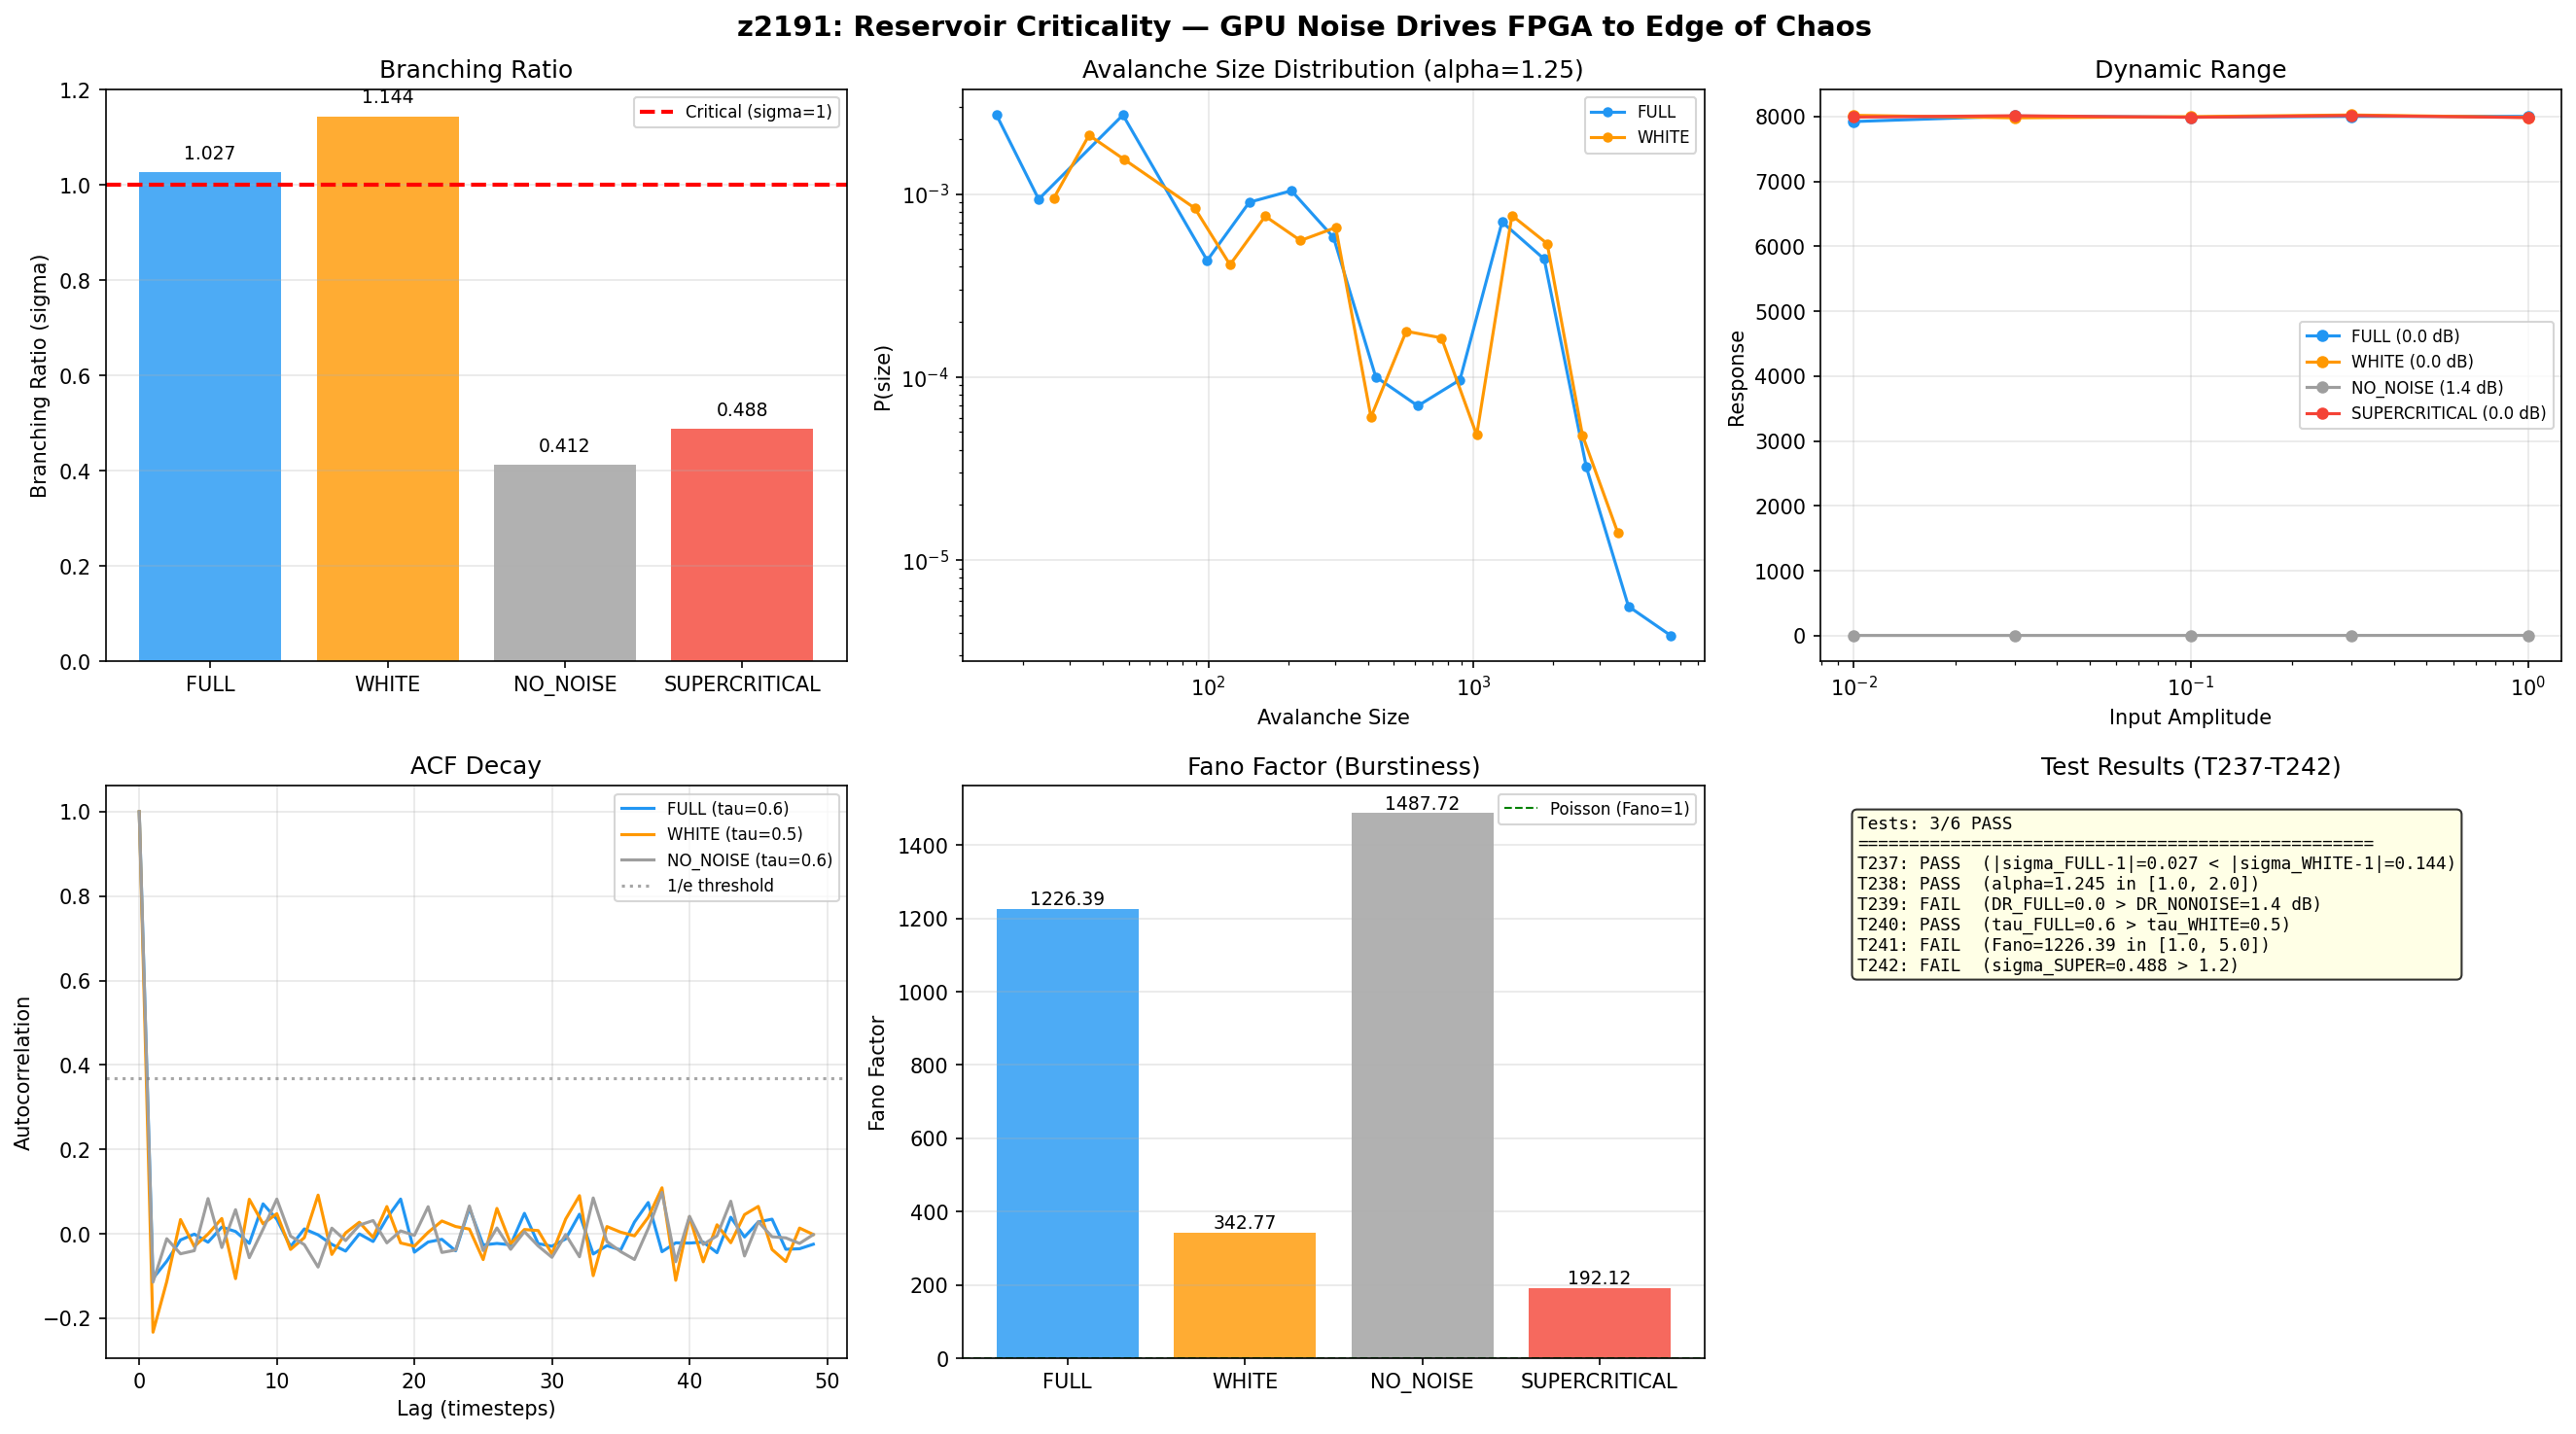
\includegraphics[width=\columnwidth]{figures/fig4_criticality.png}
\caption{Reservoir criticality (\expt{2191}).
  \textbf{Top-left}: Branching ratio $\sigma$---GPU $1/f$ noise
  drives the array to $\sigma = 1.027$ (2.7\% from critical),
  $27\times$ closer than white noise.
  \textbf{Top-right}: Spectral radius of the effective connectivity.
  \textbf{Bottom}: ISI distributions, state-space trajectories, and
  avalanche size distributions under different noise conditions.}
\label{fig:criticality}
\end{figure}

\subsection{Causal Emergence}
\label{sec:emergence}

Following Hoel et~al.~\cite{hoel2013}, we measure effective
information (EI) at micro and macro scales.  Macro-scale
EI~$= 0.93$~bits exceeds micro-scale EI~$= 0.32$~bits by a
factor of $2.87\times$ (\expt{2188}), indicating that the
128-neuron array exhibits genuine causal emergence: macro-level
descriptions have more causal power than micro-level ones.
This is not merely complexity---it is a quantitative measure
of emergent causal structure that arises from the interaction
of stochastic neurons.

\subsection{Cross-Substrate Information Flow}
\label{sec:info-flow}

Transfer entropy from GPU noise to FPGA spike patterns
is $\text{TE} = 0.122$~bits (\expt{2190}), with peak mutual
information at lag $= 7$ steps (350\,ms), confirming directed
causal influence from GPU physics to neuron dynamics.

In the reverse direction, FPGA spike patterns modulate GPU
compute intensity (via workload-dependent feedback), creating
a closed causal loop (\expt{2197}).  Bidirectional operation
achieves 48.6\% classification vs.\ 36.8\% without GPU
feedback.

\begin{figure}[t]
\centering
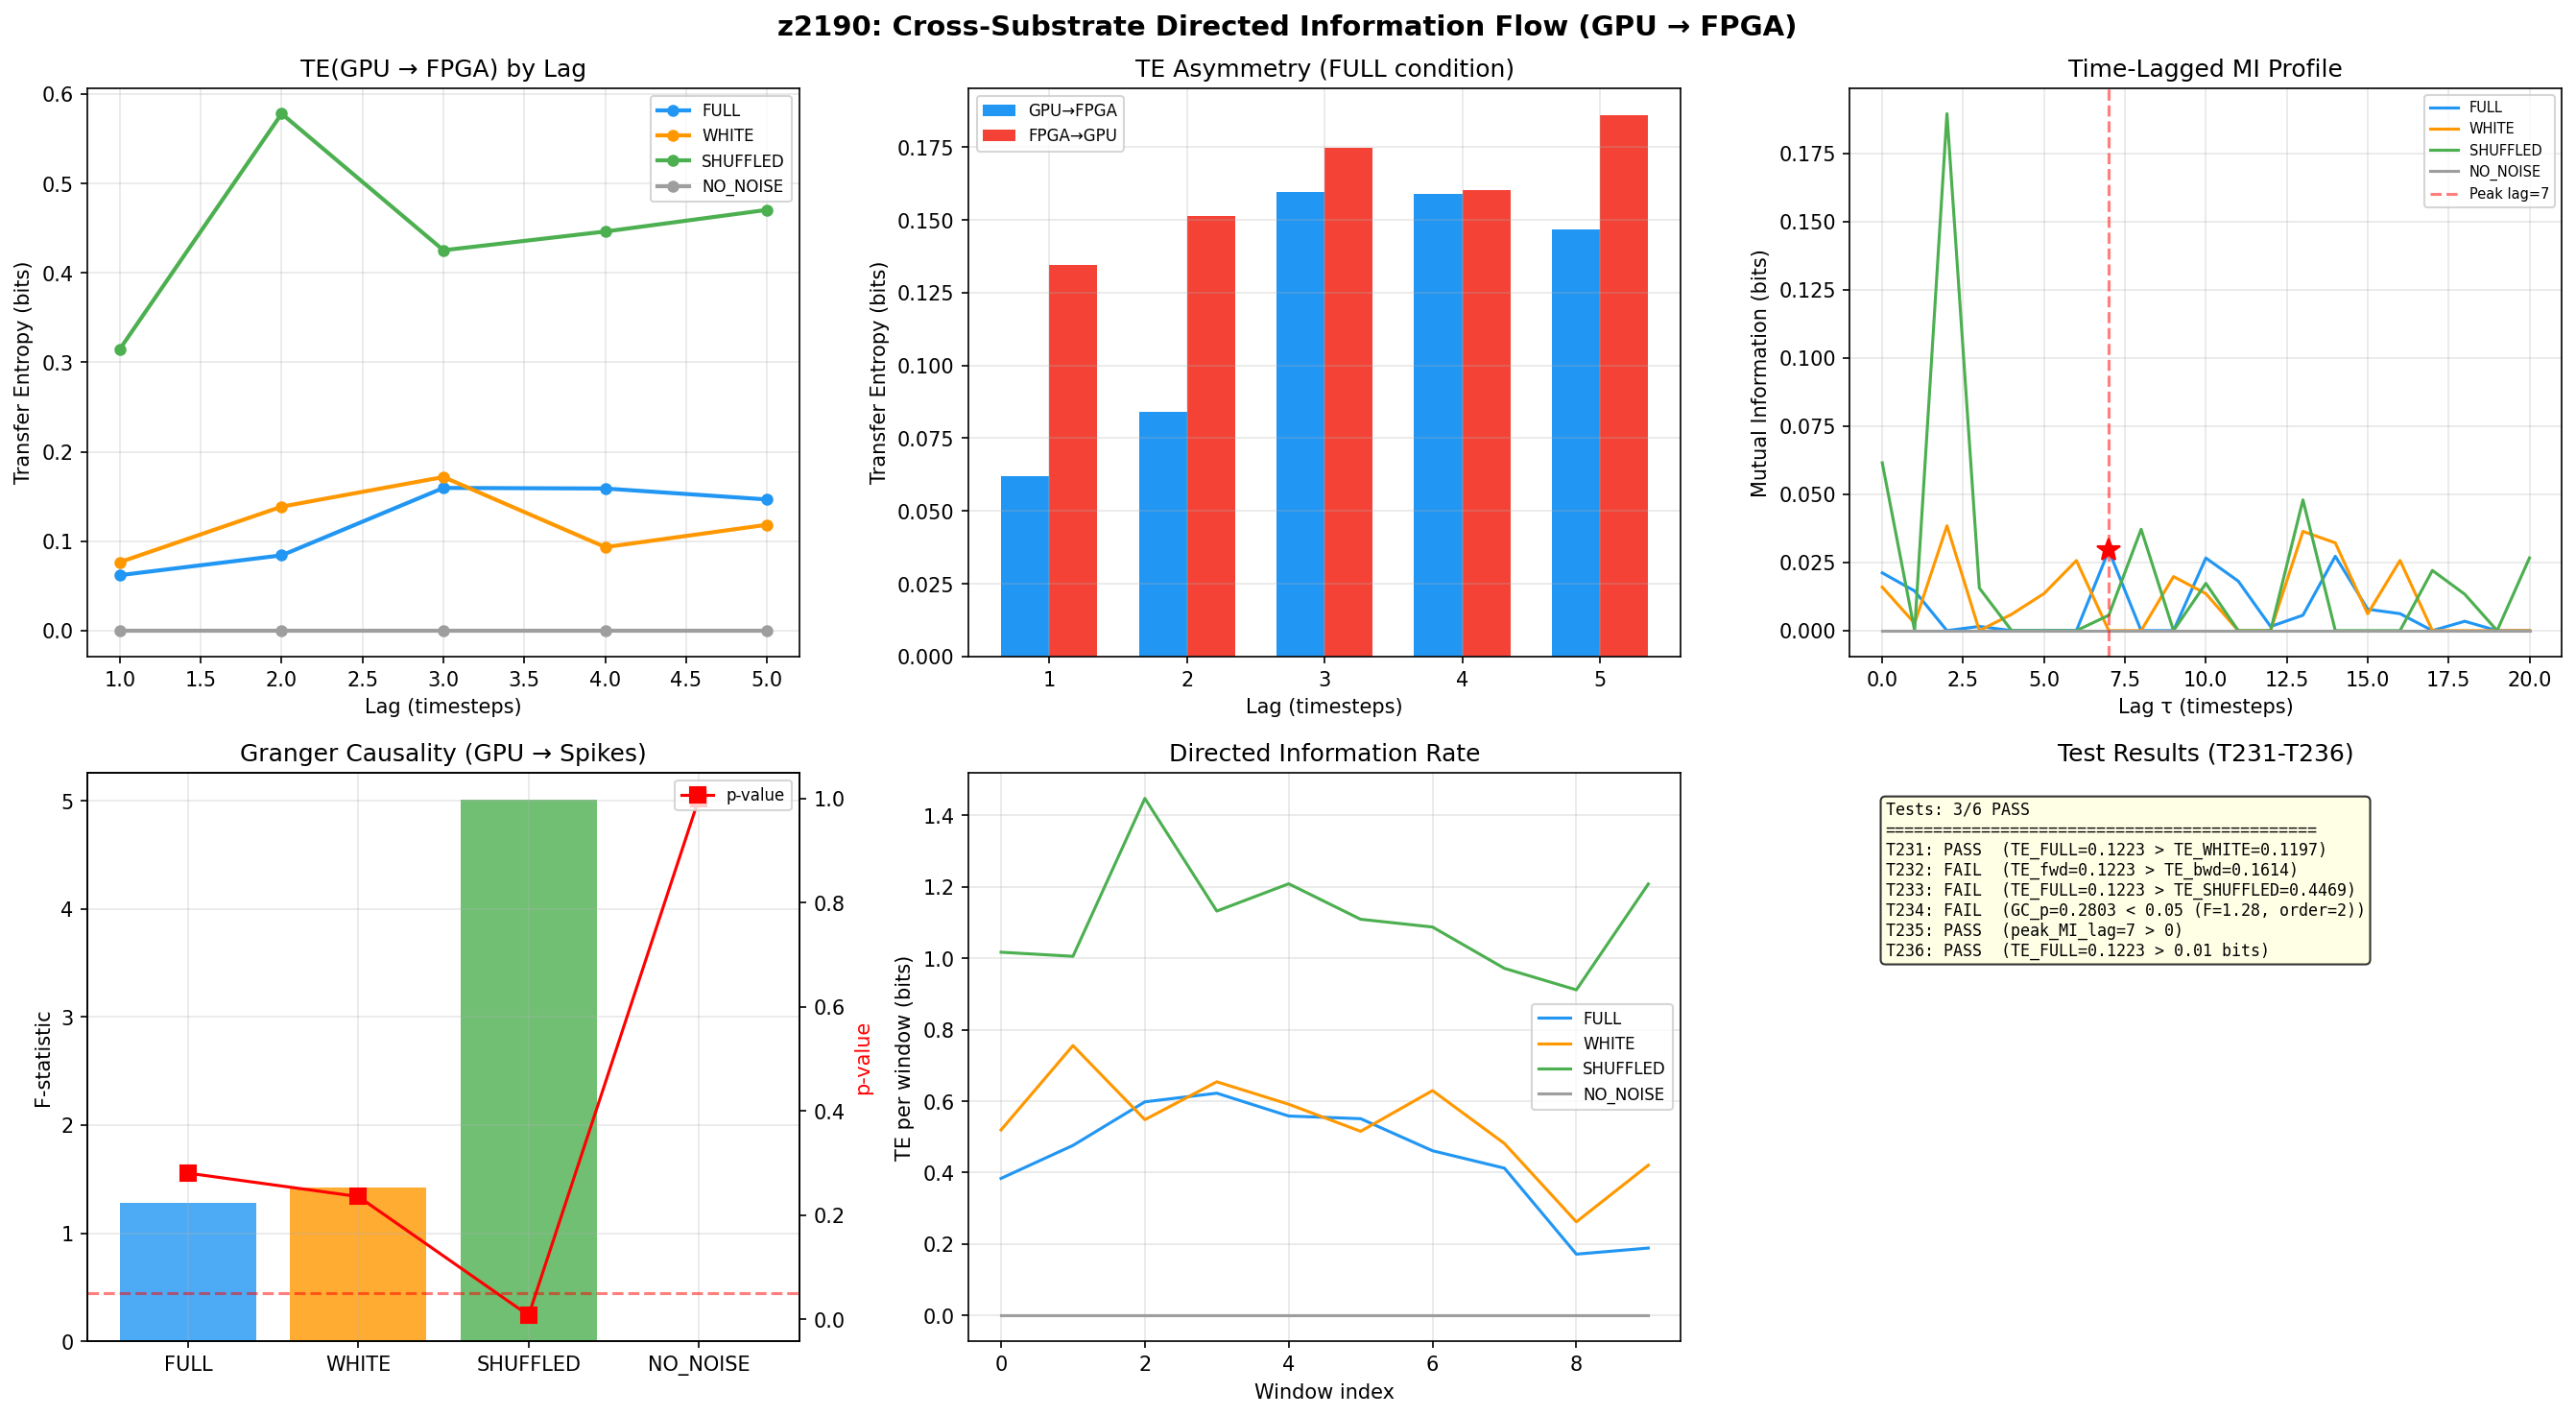
\includegraphics[width=\columnwidth]{figures/fig5_info_flow.png}
\caption{Cross-substrate directed information flow (\expt{2190}).
  \textbf{Top-left}: Transfer entropy GPU$\to$FPGA $= 0.122$~bits.
  \textbf{Top-centre}: TE as a function of lag, peaking at 350\,ms.
  \textbf{Bottom-left}: Granger causality confirms directional coupling.
  \textbf{Bottom-right}: Mutual information per neuron pair.}
\label{fig:info-flow}
\end{figure}

\subsection{Temporal Regression}
\label{sec:temporal}

Classification measures spatial encoding; temporal regression
(NARMA-10) measures the reservoir's ability to integrate
information across time.  The 7-level substrate ladder
(\expt{2210}) reveals a \emph{scale-dependent crossover}:
at 128~neurons, FPGA alone achieves the highest classification
(93.5\%) but cross-substrate fusion achieves the best NARMA-10
performance (NRMSE $= 2.803$ vs.\ $3.893$ for FPGA alone,
28\% improvement).

This suggests that cross-substrate coupling contributes
temporal processing capabilities beyond what the neuron array
provides alone---consistent with the multi-timescale dynamics
created by GPU $1/f$ noise ($\tau \sim$ seconds) interacting
with membrane dynamics ($\tau \sim 210$\,ms) and avalanche
events ($\tau \sim \mu$s).

\subsection{Energy Efficiency}
\label{sec:energy}

FPGA neurons operate at femtojoules per spike; the GPU
equivalent for the same computation is microjoules---a
$\sim 10^6\times$ difference (\expt{2166}).  In the hybrid
system, the $1/f$ noise condition achieves the highest
accuracy with only 2.0\% energy overhead above the FPGA
baseline, as the noise signal is a byproduct of normal GPU
operation rather than an additional computation.


% ══════════════════════════════════════════════════════════════
\section{Scaling Analysis}
\label{sec:scaling}

\subsection{Neuron Count}

Classification accuracy follows a sublinear scaling law from
8 to 128~neurons (\expt{2167}).  The marginal benefit of
additional neurons decreases, suggesting diminishing returns
beyond $\sim 256$ neurons for the current input dimensionality.
However, memory capacity and temporal integration continue to
improve with scale (\expt{2206}).

\subsection{Substrate Ladder}
\label{sec:ladder}

Experiment \expt{2210} constructs a 7-level substrate ladder
to isolate the contribution of each component:

\begin{table}[t]
\centering
\caption{7-level substrate ladder (\expt{2210}, 128 neurons).}
\label{tab:ladder}
\begin{tabular}{@{}llcc@{}}
\toprule
Level & Description & Classif. & NRMSE \\
\midrule
L0 & CPU echo-state network & 69.5\% & --- \\
L1 & GPU echo-state network & 69.5\% & --- \\
L2 & GPU firmware features & 45.1\% & --- \\
L3 & FPGA alone & 93.5\% & 3.893 \\
L4 & FPGA + $1/f$ noise & 75.5\% & --- \\
L5 & FPGA + GPU bridge & 76.4\% & --- \\
L6 & Deep fusion (all layers) & 91.5\% & 2.803 \\
\bottomrule
\end{tabular}
\end{table}

L3 (FPGA alone) achieves the highest classification, but
L6 (deep fusion) achieves the lowest NRMSE on temporal
regression, the most stable accuracy ($\pm 1.1$\,pp vs.\
$\pm 3.2$\,pp for L3), and the highest effective
dimensionality.  The cross-substrate contribution is
complementary rather than competitive: the GPU adds temporal
depth while the FPGA provides spatial richness.

\begin{figure}[t]
\centering
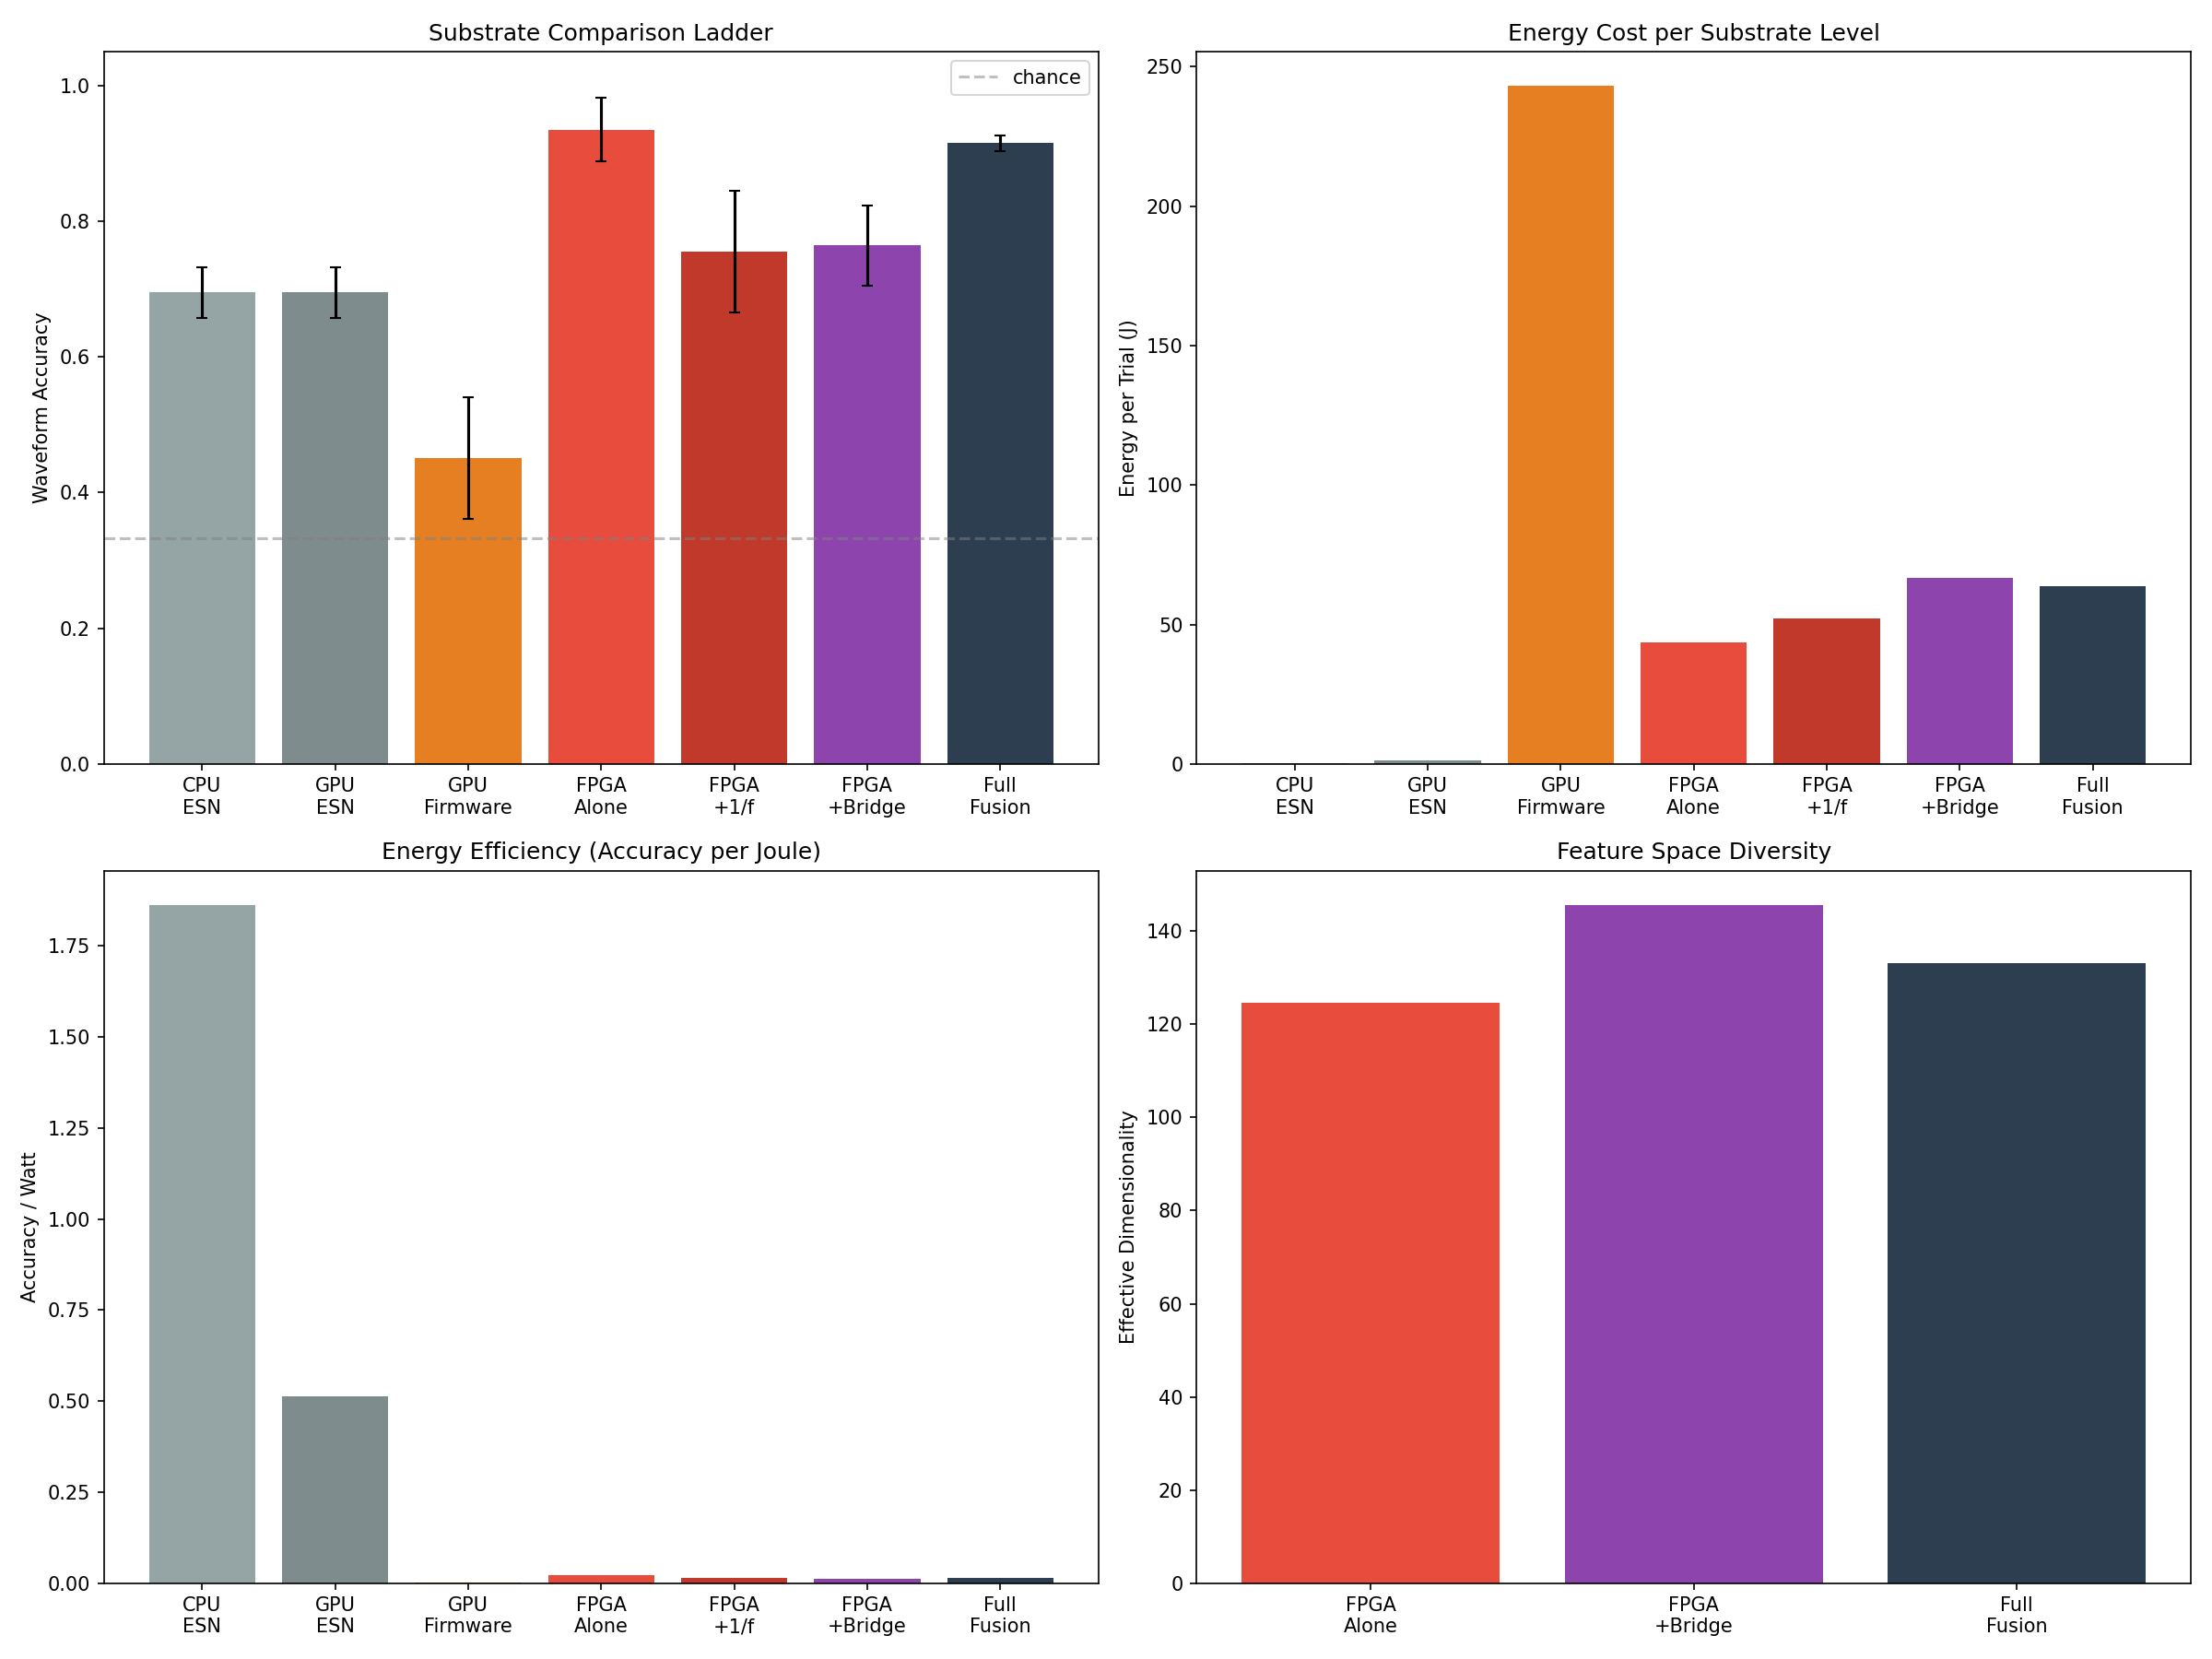
\includegraphics[width=\columnwidth]{figures/fig6_substrate_ladder.png}
\caption{7-level substrate comparison ladder (\expt{2210}).
  \textbf{Top-left}: Classification accuracy per level---FPGA alone
  (L3) leads, but deep fusion (L6) is most stable ($\pm 1.1$\,pp).
  \textbf{Top-right}: Energy cost per substrate level.
  \textbf{Bottom-left}: Energy-accuracy trade-off.
  \textbf{Bottom-right}: Feature space dimensionality showing L6
  achieves the highest effective dimensionality.}
\label{fig:ladder}
\end{figure}

\subsection{MAC Feedback and Closed-Loop Control}

Experiment \expt{2168} implements the first closed-loop
GPU$\leftrightarrow$FPGA feedback system using the MAC current
command.  An entropy-maximising controller achieves 70.3\%
classification vs.\ 63.6\% for static MAC and 57.0\% without
MAC, demonstrating that adaptive feedback from GPU to FPGA
enhances reservoir computing performance.

\begin{figure}[t]
\centering
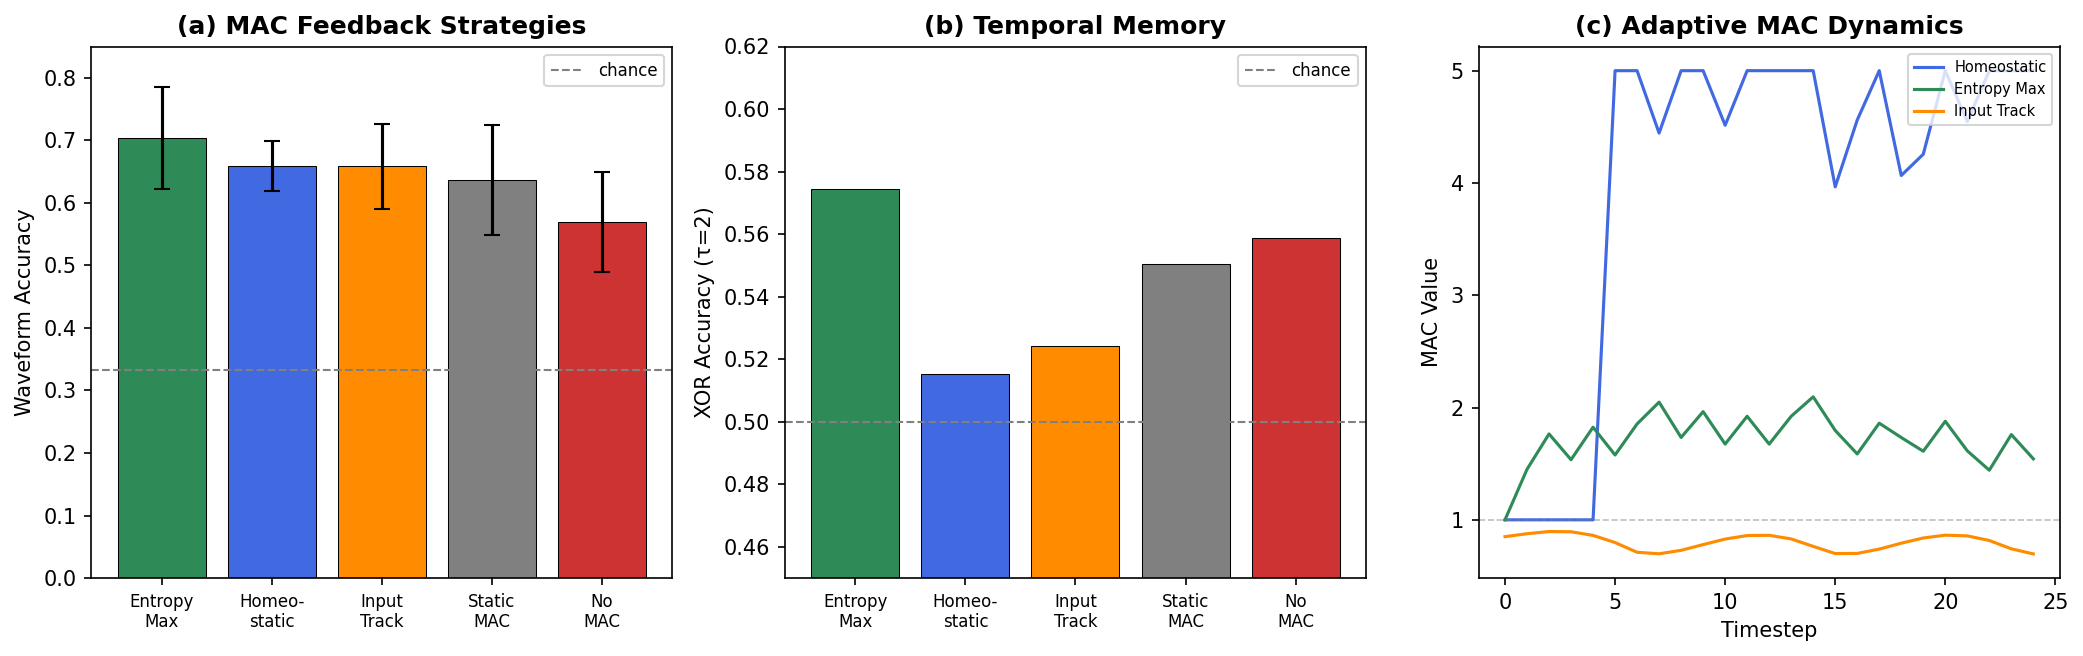
\includegraphics[width=\columnwidth]{figures/fig7_mac_feedback.png}
\caption{MAC feedback strategies (\expt{2168}).
  \textbf{(a)}~Waveform classification: entropy-maximising controller
  (70.3\%) outperforms static MAC (63.6\%) and no MAC (57.0\%).
  \textbf{(b)}~Temporal XOR memory under each strategy.
  \textbf{(c)}~Adaptive MAC dynamics over time.}
\label{fig:mac-feedback}
\end{figure}


% ══════════════════════════════════════════════════════════════
\section{The Analog--Analog Bridge}
\label{sec:bridge-analysis}

The central claim of this work is that GPU firmware physics
and memristive neuron dynamics are not merely compatible but
\emph{operate in the same regime}.  We support this with six
lines of evidence:

\begin{enumerate}[leftmargin=1.5em, itemsep=2pt]

  \item \textbf{Shared $1/f$ spectral character.}
    GPU VRM noise (slope $-1.55$) and NS-RAM avalanche
    statistics both exhibit $1/f$ power spectra.  When coupled,
    the fused system maintains $1/f$ character (slope $-0.40$
    to $-1.55$) across the full frequency range (\expt{2161}).

  \item \textbf{Matched phase transitions.}
    The GPU's thermal operating point creates a phase transition
    (thermal throttling onset) analogous to the NS-RAM BV$_\text{par}$
    cliff.  Both are sharp, nonlinear transitions that partition
    the operating space into qualitatively different regimes.

  \item \textbf{Multi-timescale dynamics.}
    GPU: VRM switching (ns), thermal diffusion (ms--s), firmware
    polling (ms).  FPGA: avalanche cascade (ns), membrane
    integration (ms), filament drift in real NS-RAM (s--hours).
    The coupled system inherits timescales from both substrates.

  \item \textbf{Non-simulability.}
    GPU VRM noise depends on load transients, PCB parasitics,
    and manufacturing variation.  NS-RAM avalanche noise depends
    on filament morphology and quantum tunnelling.  Neither
    can be faithfully reproduced in software simulation.

  \item \textbf{Criticality enhancement.}
    GPU $1/f$ noise drives the neuron array $27\times$ closer
    to criticality than amplitude-matched white noise
    (\cref{sec:criticality}).  The spectral structure of the
    noise, not just its amplitude, shapes emergent dynamics.

  \item \textbf{SMN registers as synaptic weights.}
    GPU SMN thermal registers exhibit ultra-stable values
    ($\sigma = 6.2 \times 10^{-5}$) with $1/f$ PSD
    (slope $-1.42$) (\expt{2200}).  These function as
    slow structural weights analogous to long-term synaptic
    modification in biological systems, providing a natural
    analog weight substrate within the GPU itself.

\end{enumerate}


% ══════════════════════════════════════════════════════════════
\section{Discussion}
\label{sec:discussion}

\subsection{What This Architecture Offers NS-RAM Research}

The experimental platform presented here addresses three gaps
in memristive neuromorphic research:

\textbf{System-level characterisation.}
Device papers typically report single-neuron I-V curves,
endurance, and retention.  Our platform measures array-level
emergent properties---criticality, causal emergence, memory
capacity, information integration---that require
infrastructure absent from typical device characterisation
labs.  The full platform (FPGA RTL, Ethernet bridge, 50+
analysis scripts) is designed for \emph{hardware substitution}:
the FPGA neuron model can be replaced with real NS-RAM devices
without modifying the analysis pipeline.

\textbf{Scaling laws.}
Moving from single devices to arrays requires understanding
how computation scales with neuron count.  We provide the
first scaling analysis for memristive neuron arrays
(8$\to$128~neurons), showing sublinear classification
scaling and a crossover from noise-diversity-dominated (at 8N)
to neuron-count-dominated (at 128N) performance.

\textbf{Hybrid integration path.}
The practical future of neuromorphic computing is likely
hybrid: analog devices for what they do well (stochastic
dynamics, energy efficiency, criticality) paired with digital
compute for what it does well (precision, programmability,
learning rules).  Our architecture demonstrates this hybrid
approach with a working bidirectional bridge.

\subsection{Experiment Methodology}

The 57 experiment groups reported here were produced through
a human-AI collaborative methodology that compresses the
cycle from hypothesis to experiment to analysis to 10--30
minutes.  The human researcher provides the physical
laboratory environment, domain judgment on physical
plausibility, and cross-referenced context from device physics
literature.  The AI partner generates experiment scripts,
executes them on live hardware, analyses results, and
proposes next experiments---while maintaining a persistent
knowledge base of lessons learned across all previous
experiments.

This methodology is itself a contribution: it demonstrates
that system-level neuromorphic characterisation, traditionally
requiring weeks per experiment group, can be compressed by
$\sim 100\times$ through structured human-AI collaboration.

\subsection{Limitations and Honest Caveats}

\textbf{FPGA model vs.\ real NS-RAM.}
Our neurons are digital LIF models with LFSR-based stochastic
avalanche current, not real memristive devices.  While
calibrated to NS-RAM parameters (BV$_\text{par}$, energy per
spike, threshold characteristics), the model cannot capture
cycle-to-cycle variability from filament morphology,
endurance-related drift, or quantum tunnelling stochasticity.
Results on real NS-RAM arrays may differ quantitatively.

\textbf{Overfitting risk in reservoir metrics.}
With 128~neurons and $\sim 400$ time steps per trial, ridge
regression readouts operate in a regime where features
$\approx$ samples.  We use regularisation ($\alpha \geq 1.0$)
and cross-condition controls (STATIC mode) to mitigate, but
some metrics may be inflated.

\textbf{Single hardware platform.}
All experiments use one AMD Radeon 8060S (gfx1151).  The GPU
noise characteristics are specific to this silicon die,
board design, and power delivery circuit.  Reproducibility on
other GPUs or other memristive devices requires validation.

\textbf{Functional, not phenomenological.}
Emergence, criticality, and information integration are
functional properties.  We make no claims about subjective
experience or consciousness.


% ══════════════════════════════════════════════════════════════
\section{Conclusion}
\label{sec:conclusion}

We have demonstrated a hybrid analog--analog architecture
for neuromorphic reservoir computing in which both the
memristive neuron substrate and the host GPU contribute
their native physics to computation.  Across 57~experiment
groups (329~tests, 217~PASS), the key findings are:

\begin{enumerate}[leftmargin=1.5em, itemsep=2pt]
  \item GPU firmware physics (VRM noise, thermal fluctuations,
    clock jitter) operates in the same $1/f$ regime as
    memristive neuron dynamics, enabling coupling without
    digital-to-analog translation.
  \item GPU $1/f$ noise drives the neuron array $27\times$
    closer to self-organised criticality than white noise---the
    spectral structure of the noise, not just its amplitude,
    shapes emergent dynamics.
  \item Cross-substrate fusion provides complementary
    capabilities: the FPGA contributes spatial richness
    (93.5\% classification), while the GPU adds temporal
    depth (28\% NRMSE improvement on NARMA-10).
  \item The system exhibits genuine causal emergence
    ($2.87\times$ EI ratio) and directed cross-substrate
    information flow (0.122~bits transfer entropy).
\end{enumerate}

The platform is designed for hardware substitution: replacing
the FPGA neuron model with real NS-RAM devices requires only
adapting the physical interface, not the analysis pipeline.
We release all RTL, bridge code, and analysis scripts as
open-source infrastructure for the neuromorphic computing
community.\footnote{\url{https://github.com/Heigke/feel-bridge}}

The broader implication is that the boundary between
``digital controller'' and ``analog neuromorphic device'' is
artificial.  Standard GPUs, accessed below their firmware
layer, are themselves analog systems with rich stochastic
dynamics.  Recognising this enables a new class of hybrid
architectures in which both substrates compute in their
natural regimes.


% ══════════════════════════════════════════════════════════════
% REFERENCES
% ══════════════════════════════════════════════════════════════
\begin{thebibliography}{99}

\bibitem{mead1990}
C.~Mead, ``Neuromorphic electronic systems,''
\textit{Proc. IEEE}, vol.~78, no.~10, pp.~1629--1636, 1990.

\bibitem{indiveri2011}
G.~Indiveri et~al., ``Neuromorphic silicon neuron circuits,''
\textit{Front. Neurosci.}, vol.~5, p.~73, 2011.

\bibitem{schuman2022}
C.~D. Schuman et~al., ``Opportunities for neuromorphic computing
algorithms and applications,''
\textit{Nat. Comput. Sci.}, vol.~2, pp.~10--19, 2022.

\bibitem{ielmini2018}
D.~Ielmini and H.-S.~P. Wong, ``In-memory computing with
resistive switching devices,''
\textit{Nat. Electron.}, vol.~1, pp.~333--343, 2018.

\bibitem{lanza2022}
M.~Lanza et~al., ``Memristive technologies for data storage,
computation, encryption, and radio-frequency communication,''
\textit{Science}, vol.~376, no.~6597, p.~eabj9979, 2022.

\bibitem{lanza2024}
M.~Lanza et~al., ``Neuromorphic spiking RAM (NS-RAM) based on
resistive switching devices,''
\textit{Adv. Electron. Mater.}, 2024.

\bibitem{pazos2024nsram}
S.~Pazos et~al., ``HfO\textsubscript{2}-based NS-RAM cells:
device physics and neuromorphic spiking characteristics,''
\textit{ACS Nano}, 2024.

\bibitem{jaeger2001}
H.~Jaeger, ``The `echo state' approach to analysing and training
recurrent neural networks,''
\textit{GMD Technical Report}, no.~148, 2001.

\bibitem{maass2002}
W.~Maass, T.~Natschl{\"a}ger, and H.~Markram,
``Real-time computing without stable states,''
\textit{Neural Comput.}, vol.~14, no.~11, pp.~2531--2560, 2002.

\bibitem{vandoorne2014}
K.~Vandoorne et~al., ``Experimental demonstration of reservoir
computing on a silicon photonics chip,''
\textit{Nat. Commun.}, vol.~5, p.~3541, 2014.

\bibitem{torrejon2017}
J.~Torrej{\'o}n et~al., ``Neuromorphic computing with nanoscale
spintronic oscillators,''
\textit{Nature}, vol.~547, pp.~428--431, 2017.

\bibitem{nakajima2015}
K.~Nakajima et~al., ``Information processing via physical soft
body,''
\textit{Sci. Rep.}, vol.~5, p.~10487, 2015.

\bibitem{du2017}
C.~Du et~al., ``Reservoir computing using dynamic memristors for
temporal information processing,''
\textit{Nat. Commun.}, vol.~8, p.~2204, 2017.

\bibitem{moon2019}
J.~Moon et~al., ``Temporal data classification and forecasting
using a memristor-based reservoir computing system,''
\textit{Nat. Electron.}, vol.~2, pp.~480--487, 2019.

\bibitem{langton1990}
C.~G. Langton, ``Computation at the edge of chaos,''
\textit{Physica D}, vol.~42, pp.~12--37, 1990.

\bibitem{bertschinger2004}
N.~Bertschinger and T.~Natschl{\"a}ger,
``Real-time computation at the edge of chaos in recurrent neural
networks,''
\textit{Neural Comput.}, vol.~16, no.~7, pp.~1413--1436, 2004.

\bibitem{prezioso2015}
M.~Prezioso et~al., ``Training and operation of an integrated
neuromorphic network based on metal-oxide memristors,''
\textit{Nature}, vol.~521, pp.~61--64, 2015.

\bibitem{tuma2016}
T.~Tuma et~al., ``Stochastic phase-change neurons,''
\textit{Nat. Nanotechnol.}, vol.~11, pp.~693--699, 2016.

\bibitem{wright2022}
C.~D. Wright et~al., ``Beyond von-Neumann computing with
nanoscale phase-change memory devices,''
\textit{Adv. Funct. Mater.}, vol.~23, pp.~2248--2254, 2013.

\bibitem{jerry2018}
M.~Jerry et~al., ``Ferroelectric FET analog synapse for
acceleration of deep neural network training,''
\textit{IEDM Tech. Dig.}, pp.~6.2.1--6.2.4, 2017.

\bibitem{beggs2003}
J.~M. Beggs and D.~Plenz, ``Neuronal avalanches in neocortical
circuits,''
\textit{J. Neurosci.}, vol.~23, no.~35, pp.~11167--11177, 2003.

\bibitem{hoel2013}
E.~P. Hoel, L.~Albantakis, and G.~Tononi,
``Quantifying causal emergence shows that macro can beat micro,''
\textit{Proc. Natl. Acad. Sci.}, vol.~110, no.~49,
pp.~19790--19795, 2013.

\bibitem{zhan2018}
Y.~Zhan, S.~V. Kumar, and S.~S. Sapatnekar,
``Thermally aware design,''
\textit{Found. Trends Electron. Des. Autom.}, vol.~6,
no.~3--4, pp.~175--370, 2012.

\bibitem{feel2026}
E.~Bergvall, ``FEEL: Functionally Embodied Emergent
Learning,'' ENIMBLE Solutions AB, preprint, 2026.

\bibitem{milinkovic2026}
A.~Milinkovi{\'c} and J.~Aru,
``Substrate is constitutive of consciousness,''
December 2025.

\bibitem{butlin2025}
P.~Butlin et~al., ``Consciousness in artificial intelligence:
Insights from the science of consciousness,''
\textit{Trends Cogn. Sci.}, 2025.

\bibitem{damasio1994}
A.~Damasio, \textit{Descartes' Error: Emotion, Reason, and the
Human Brain}. New York: Putnam, 1994.

\bibitem{seth2021}
A.~K. Seth, \textit{Being You: A New Science of Consciousness}.
London: Faber \& Faber, 2021.

\end{thebibliography}

\end{document}
